%%%%%%%%%%%%%%%%%%%%%%%%%%%%%%%%%%%%%%%%%%%%%%%%%%%%%%%%%%%%%%%%%%%%%%%%%%%%%%%%%%
\begin{frame}[fragile]\frametitle{}
\begin{center}
{\Large Docling}
\end{center}

\end{frame}

%%%%%%%%%%%%%%%%%%%%%%%%%%%%%%%%%%%%%%%%%%%%%%%%%%%%%%%%%%%
\begin{frame}[fragile]\frametitle{What is Docling?}
      \begin{itemize}
	\item Simplifies document processing across diverse formats
	\item Provides advanced PDF understanding capabilities
	\item Offers seamless integrations with generative AI ecosystem
	\item Handles complex document structures and layouts
	\item Enables unified document representation format
	\item Supports both local and cloud-based processing
	  \end{itemize}
\end{frame}

%%%%%%%%%%%%%%%%%%%%%%%%%%%%%%%%%%%%%%%%%%%%%%%%%%%%%%%%%%%
\begin{frame}[fragile]\frametitle{Key Features}
      \begin{itemize}
	\item Multi-format parsing: PDF, DOCX, PPTX, XLSX, HTML, audio files, images
	\item Advanced PDF understanding: layout, reading order, tables, formulas
	\item Unified DoclingDocument representation format
	\item Multiple export options: Markdown, HTML, DocTags, JSON
	\item Local execution for sensitive data and air-gapped environments
	\item Plug-and-play integrations: LangChain, LlamaIndex, Crew AI, Haystack
	\item Extensive OCR support for scanned documents
	\item Visual Language Models support (SmolDocling)
	\item Automatic Speech Recognition for audio files
	\item Simple command-line interface
	  \end{itemize}
\end{frame}

%%%%%%%%%%%%%%%%%%%%%%%%%%%%%%%%%%%%%%%%%%%%%%%%%%%%%%%%%%%
\begin{frame}[fragile]\frametitle{Architecture Overview}
\begin{columns}
    \begin{column}[T]{0.4\linewidth}
      \begin{itemize}
		\item Document converter selects format-specific backend
		\item Pipeline orchestrates execution with relevant options
		\item Conversion result contains DoclingDocument representation
		\item Export methods available for various output formats
		\item Serializers handle document transformation
		\item Chunkers enable document segmentation
	  \end{itemize}

    \end{column}
    \begin{column}[T]{0.6\linewidth}
		\begin{center}
		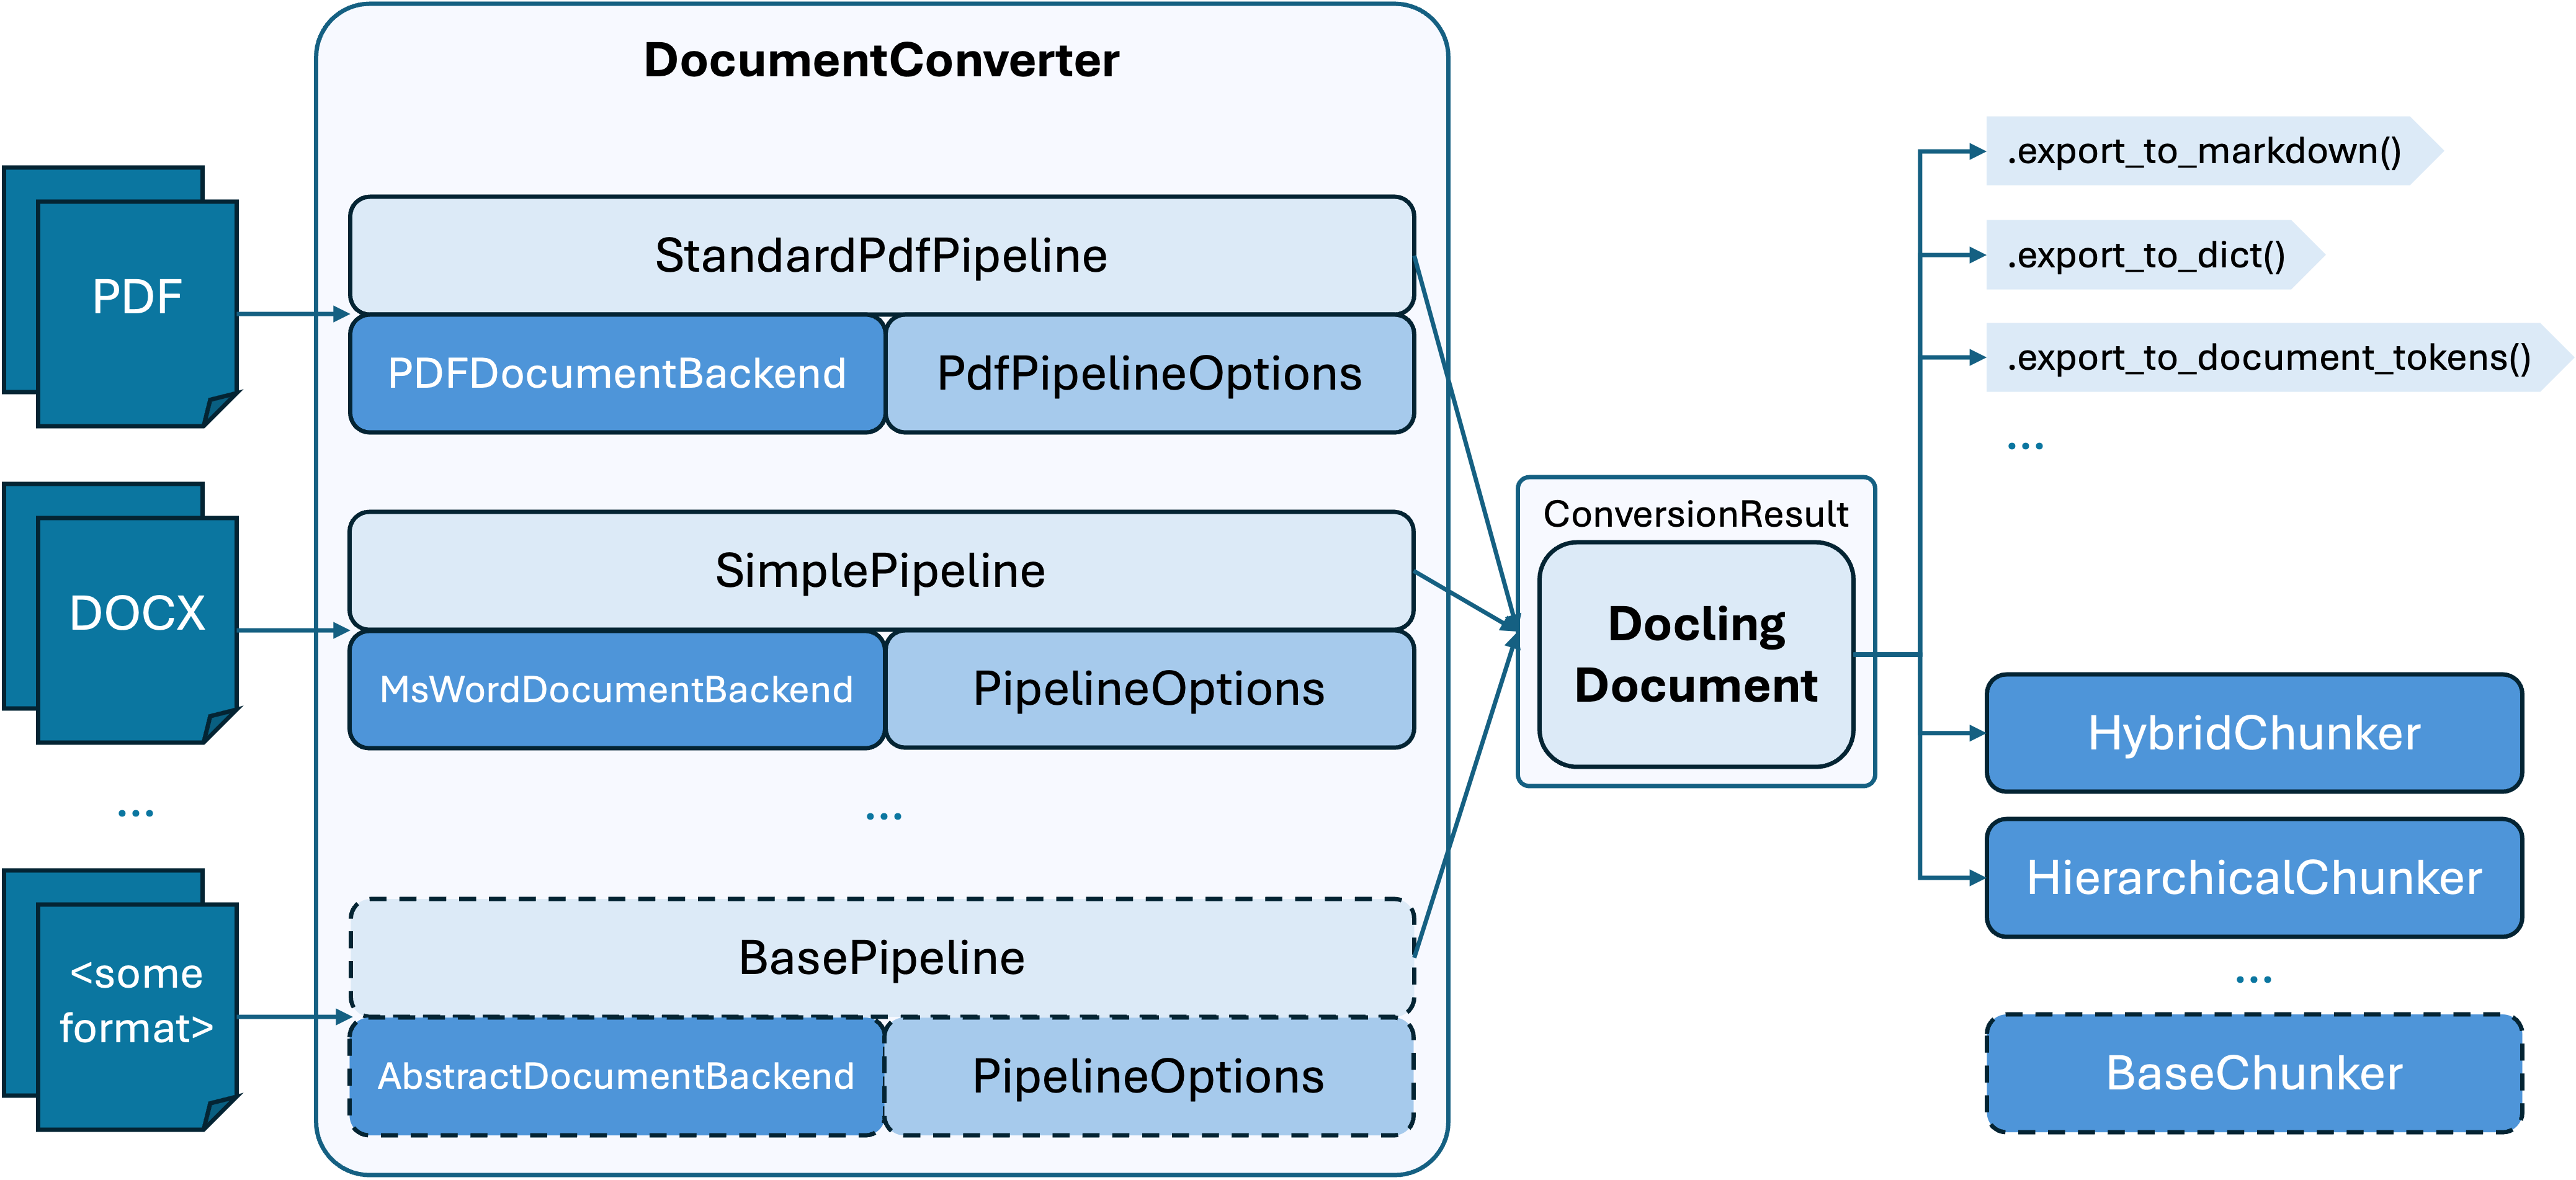
\includegraphics[width=\linewidth,keepaspectratio]{docling1}
		\end{center}	
    \end{column}
  \end{columns}
\end{frame}

%%%%%%%%%%%%%%%%%%%%%%%%%%%%%%%%%%%%%%%%%%%%%%%%%%%%%%%%%%%
\begin{frame}[fragile]\frametitle{DoclingDocument Structure}
      \begin{itemize}
	\item Unified document representation using Pydantic datatype
	\item Expresses text, tables, pictures, and hierarchical sections
	\item Distinguishes main body from headers/footers (furniture)
	\item Includes layout information with bounding boxes
	\item Maintains provenance information for traceability
	\item Supports disambiguation between content types
	\item Enables structured document analysis and processing
	  \end{itemize}
\end{frame}

%%%%%%%%%%%%%%%%%%%%%%%%%%%%%%%%%%%%%%%%%%%%%%%%%%%%%%%%%%%
\begin{frame}[fragile]\frametitle{Document Content Categories}
      \begin{itemize}
	\item \textbf{Content Items:}
	\begin{itemize}
		\item texts: All text representations (paragraphs, headings, equations)
		\item tables: Table structures with annotations
		\item pictures: Image content with metadata
		\item key\_value\_items: Structured data pairs
	\end{itemize}
	\item \textbf{Content Structure:}
	\begin{itemize}
		\item body: Main document tree structure
		\item furniture: Headers, footers, and non-body content
		\item groups: Container items for organizing content
	\end{itemize}
	\item All items inherit from DocItem type with JSON pointer references
	  \end{itemize}
\end{frame}

%%%%%%%%%%%%%%%%%%%%%%%%%%%%%%%%%%%%%%%%%%%%%%%%%%%%%%%%%%%
\begin{frame}[fragile]\frametitle{Document Hierarchy}

      \begin{itemize}
		\item Reading order maintained through body tree structure
		\item Items nested hierarchically under parent elements
		\item Children ordered sequentially within each tree node
		\item Page-level organization with title-based grouping
		\item JSON pointer system for parent-child relationships
	  \end{itemize}


		\begin{center}
		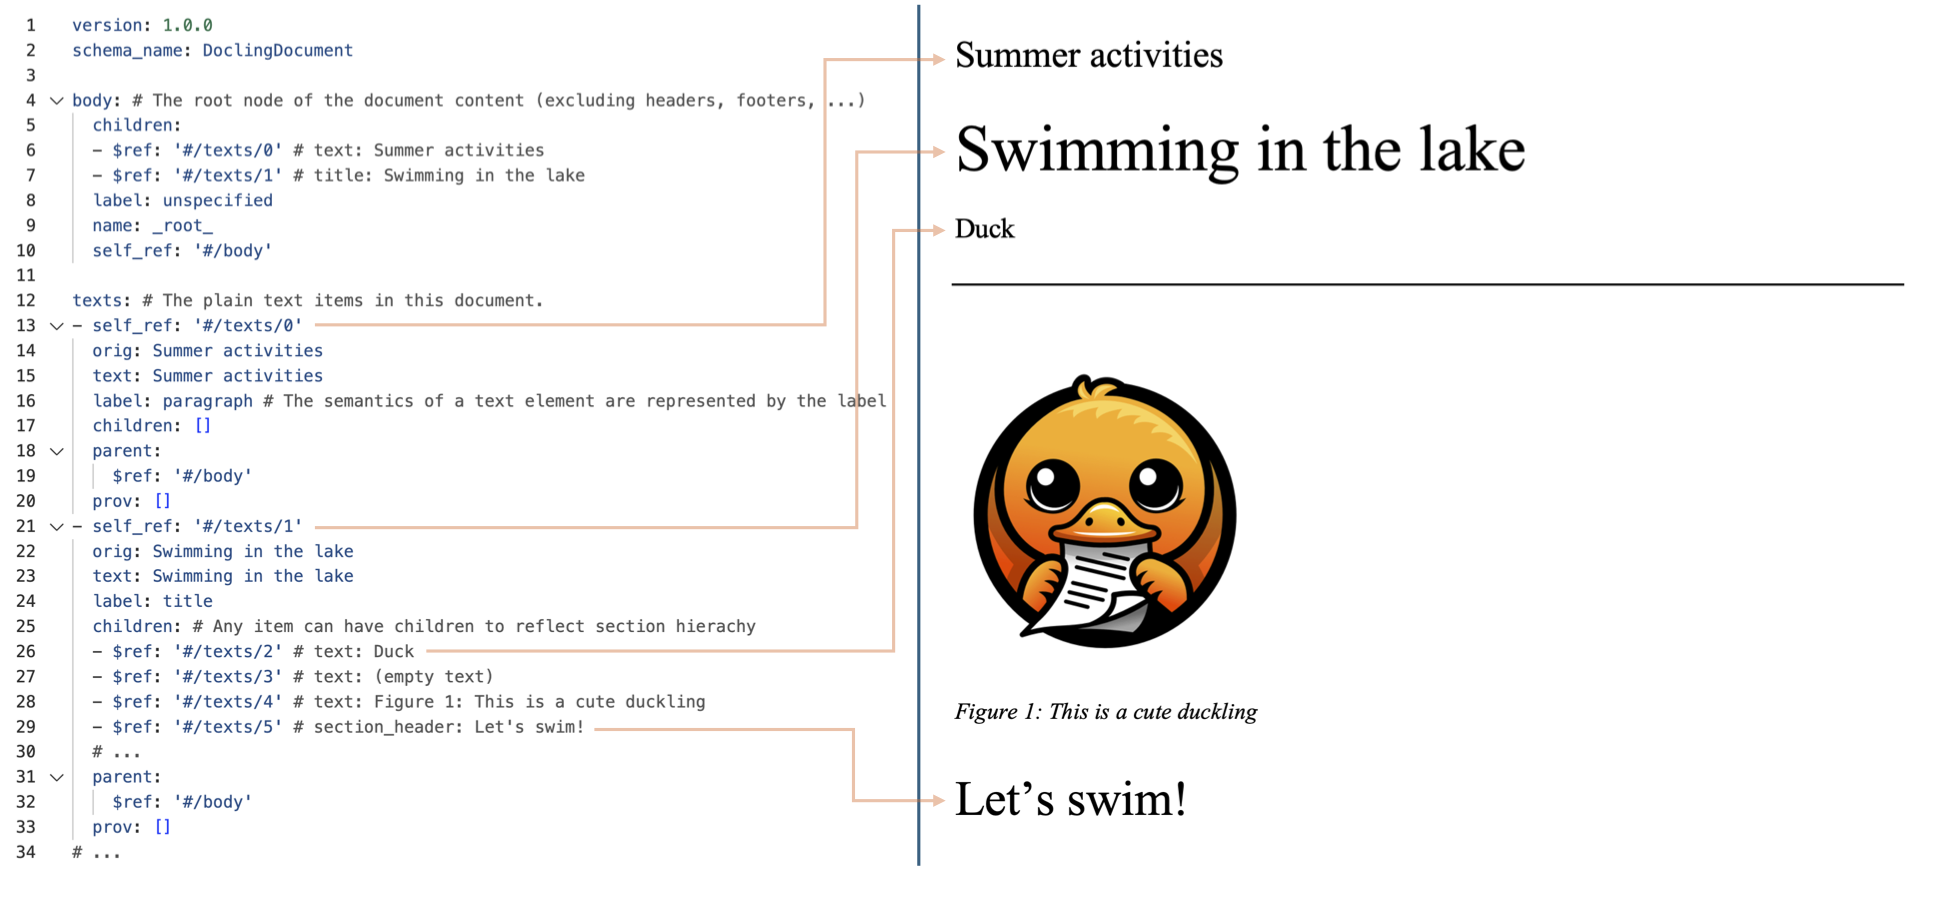
\includegraphics[width=0.8\linewidth,keepaspectratio]{docling2}
		\end{center}	

\end{frame}

%%%%%%%%%%%%%%%%%%%%%%%%%%%%%%%%%%%%%%%%%%%%%%%%%%%%%%%%%%%
\begin{frame}[fragile]\frametitle{Content Grouping}

      \begin{itemize}
		\item Items grouped under section headings
		\item Children include both text items and group containers
		\item List elements organized within group structures
		\item Group items stored in top-level groups field
		\item Hierarchical nesting preserves document structure
	  \end{itemize}

		\begin{center}
		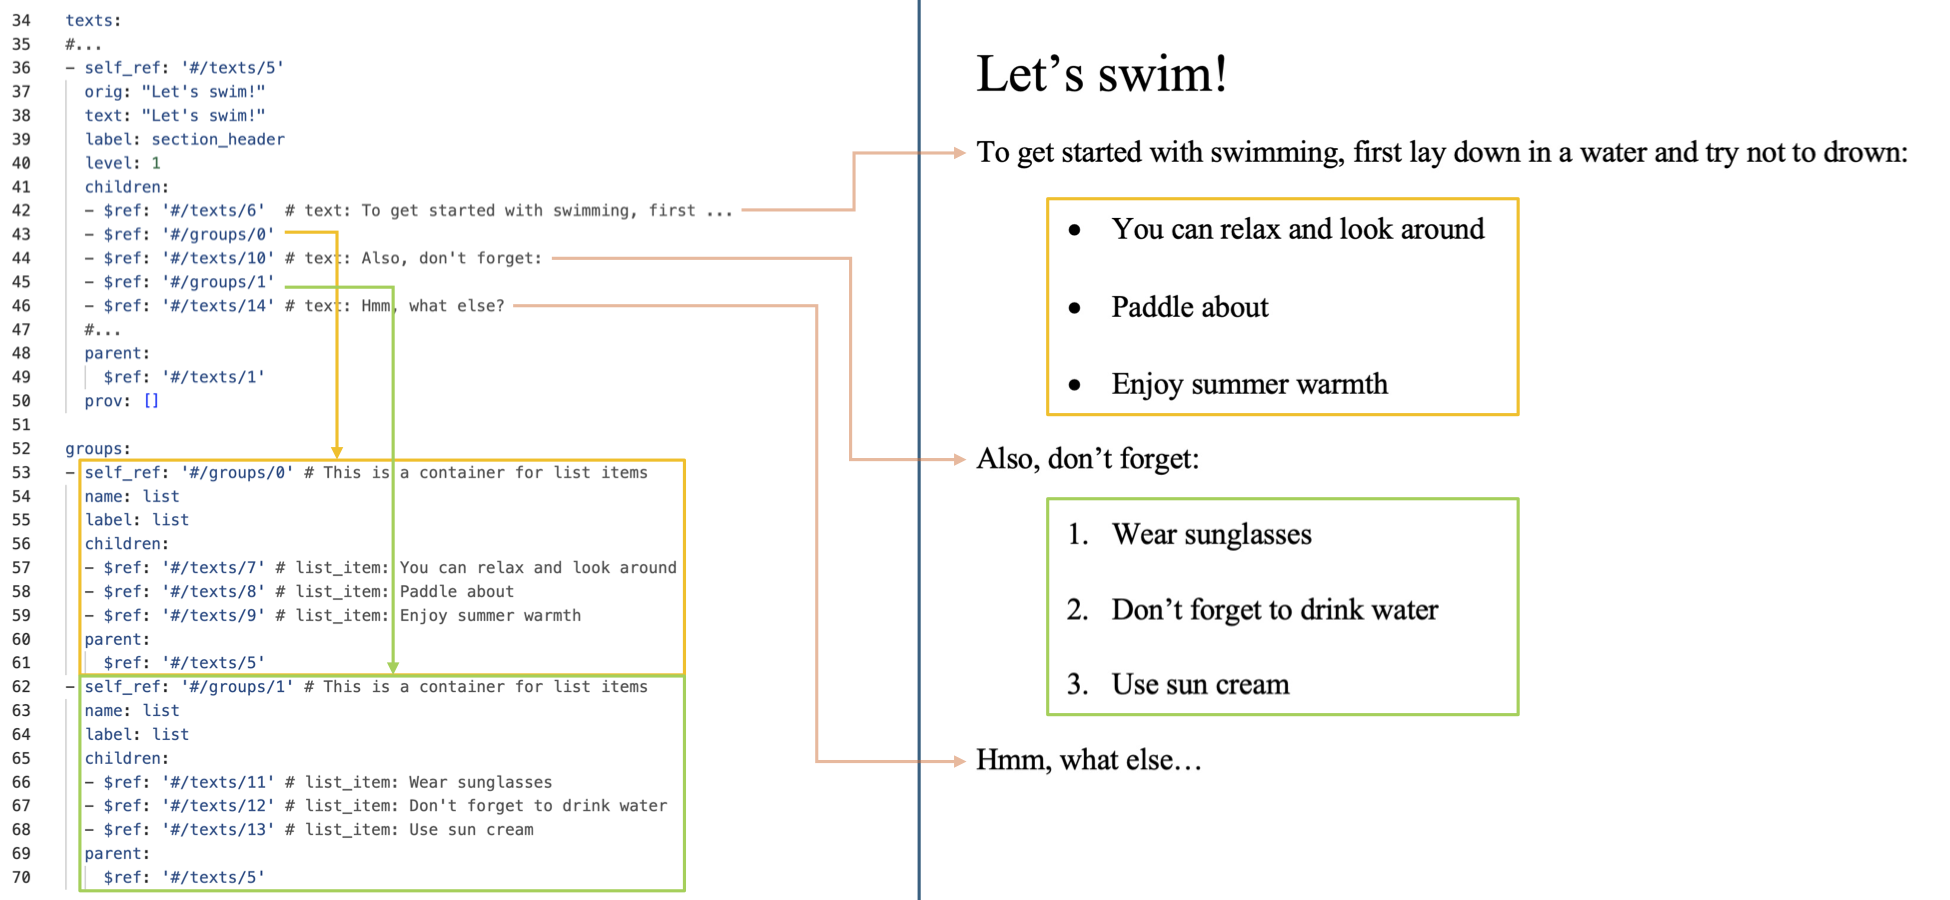
\includegraphics[width=0.8\linewidth,keepaspectratio]{docling3}
		\end{center}	

\end{frame}

%%%%%%%%%%%%%%%%%%%%%%%%%%%%%%%%%%%%%%%%%%%%%%%%%%%%%%%%%%%
\begin{frame}[fragile]\frametitle{Serialization Framework}
      \begin{itemize}
	\item Document serializer converts DoclingDocument to textual format
	\item Component serializers: text, table, picture, list, inline
	\item Serializer provider abstracts serialization strategy
	\item Base classes enable flexibility and out-of-the-box utility
	\item Hierarchy includes BaseDocSerializer and specific subclasses
	\item serialize() method returns text with contribution metadata
	\item Predefined serializers for Markdown, HTML, DocTags
	\item Export methods act as user-friendly shortcuts
	  \end{itemize}
\end{frame}

%%%%%%%%%%%%%%%%%%%%%%%%%%%%%%%%%%%%%%%%%%%%%%%%%%%%%%%%%%%
\begin{frame}[fragile]\frametitle{Confidence Scores}
      \begin{itemize}
	\item Quantitative assessment of document conversion quality
	\item Numerical scores from 0.0 to 1.0 (higher = better quality)
	\item Quality grades: POOR, FAIR, GOOD, EXCELLENT
	\item Helps identify documents requiring manual review
	\item Enables adjustment of conversion pipelines per document type
	\item Supports confidence thresholds for batch processing
	\item Early detection of potential conversion issues
	\item Available in ConversionResult confidence field
	  \end{itemize}
\end{frame}

%%%%%%%%%%%%%%%%%%%%%%%%%%%%%%%%%%%%%%%%%%%%%%%%%%%%%%%%%%%
\begin{frame}[fragile]\frametitle{Confidence Score Components}
      \begin{itemize}
	\item \textbf{Four component scores:}
	\begin{itemize}
		\item layout\_score: Document element recognition quality
		\item ocr\_score: OCR-extracted content quality
		\item parse\_score: 10th percentile of digital text cells
		\item table\_score: Table extraction quality (in development)
	\end{itemize}
	\item \textbf{Summary grades:}
	\begin{itemize}
		\item mean\_grade: Average of four component scores
		\item low\_grade: 5th percentile score (worst areas)
	\end{itemize}
	\item Available at both page-level and document-level
	  \end{itemize}
\end{frame}

%%%%%%%%%%%%%%%%%%%%%%%%%%%%%%%%%%%%%%%%%%%%%%%%%%%%%%%%%%%
\begin{frame}[fragile]\frametitle{Confidence Example}
\begin{columns}
    \begin{column}[T]{0.4\linewidth}
      \begin{itemize}
		\item Page-level scores stored in pages field
		\item Document-level scores as averages in root ConfidenceReport
		\item Numerical values for internal processing
		\item Categorical grades for user interpretation
		\item Comprehensive quality assessment framework
	  \end{itemize}

    \end{column}
    \begin{column}[T]{0.6\linewidth}
		\begin{center}
		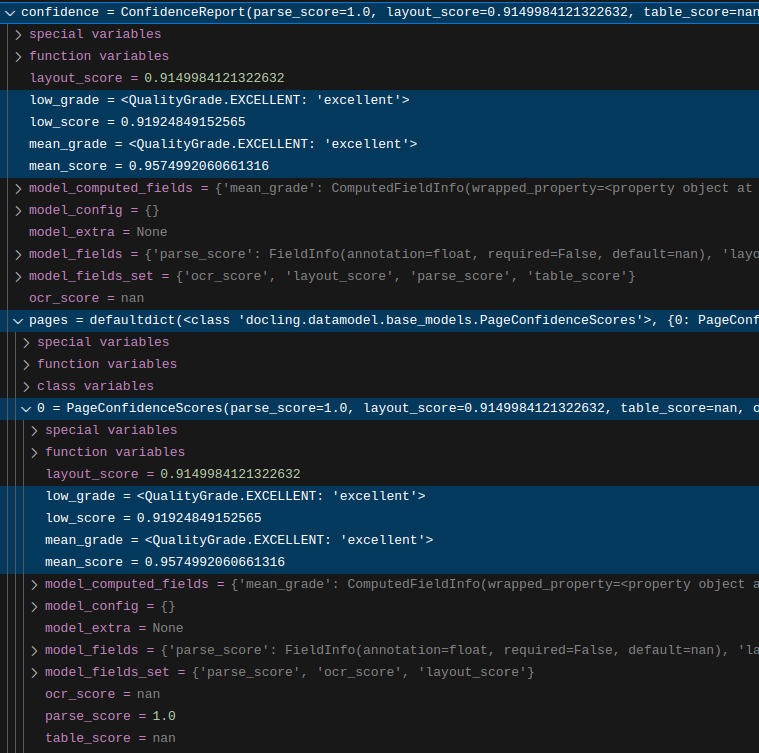
\includegraphics[width=\linewidth,keepaspectratio]{docling4}
		\end{center}	
    \end{column}
  \end{columns}
\end{frame}

%%%%%%%%%%%%%%%%%%%%%%%%%%%%%%%%%%%%%%%%%%%%%%%%%%%%%%%%%%%
\begin{frame}[fragile]\frametitle{Chunking Framework}
      \begin{itemize}
	\item Chunker abstracts document segmentation from DoclingDocument
	\item Returns stream of chunks with metadata
	\item Base class hierarchy: BaseChunker and specific subclasses
	\item Integration with LlamaIndex and other gen AI frameworks
	\item chunk() method returns iterator of BaseChunk objects
	\item contextualize() method enriches chunks with metadata
	\item Enables flexible downstream application integration
	\item Supports embedding model and generation model feeding
	  \end{itemize}
\end{frame}

%%%%%%%%%%%%%%%%%%%%%%%%%%%%%%%%%%%%%%%%%%%%%%%%%%%%%%%%%%%
\begin{frame}[fragile]\frametitle{Chunking Implementations}
      \begin{itemize}
	\item \textbf{Hybrid Chunker:}
	\begin{itemize}
		\item Tokenization-aware refinements on hierarchical chunks
		\item Splits oversized chunks based on token limits
		\item Merges undersized successive chunks with same headings
		\item User-configurable merge\_peers parameter
	\end{itemize}
	\item \textbf{Hierarchical Chunker:}
	\begin{itemize}
		\item Uses document structure for element-based chunking  
		\item Merges list items by default (configurable)
		\item Attaches relevant metadata including headers and captions
	\end{itemize}
	  \end{itemize}
	  
\begin{lstlisting}
from docling.document_converter import DocumentConverter
from docling.chunking import HybridChunker

doc = DocumentConverter().convert(source=DOC_SOURCE).document
chunker = HybridChunker()
chunk_iter = chunker.chunk(dl_doc=doc)

for i, chunk in enumerate(chunk_iter):
    print(f"=== {i} ===")
    print(f"chunk.text:\n{f'{chunk.text[:300]}'!r}")
    enriched_text = chunker.contextualize(chunk=chunk)
    print(f"chunker.contextualize(chunk):\n{f'{enriched_text[:300]}'!r}")
    print()
\end{lstlisting}		  
\end{frame}

%%%%%%%%%%%%%%%%%%%%%%%%%%%%%%%%%%%%%%%%%%%%%%%%%%%%%%%%%%%
\begin{frame}[fragile]\frametitle{Basic Table Serialization}
Inspect the first chunk containing a table — using the default serialization strategy (first example)

	  
\begin{lstlisting}
chunker = HybridChunker(tokenizer=tokenizer)

chunk_iter = chunker.chunk(dl_doc=doc)

chunks = list(chunk_iter)
i, chunk = find_n_th_chunk_with_label(chunks, n=0, label=DocItemLabel.TABLE)
print_chunk(
    chunks=chunks,
    chunk_pos=i,
)

\end{lstlisting}		  
\end{frame}

%%%%%%%%%%%%%%%%%%%%%%%%%%%%%%%%%%%%%%%%%%%%%%%%%%%%%%%%%%%
\begin{frame}[fragile]\frametitle{Advanced Table Serialization}
Specify a different table serializer that serializes tables to Markdown instead of the triplet notation used by default:
	  
\begin{lstlisting}
from docling_core.transforms.chunker.hierarchical_chunker import (
    ChunkingDocSerializer,
    ChunkingSerializerProvider,
)
from docling_core.transforms.serializer.markdown import MarkdownTableSerializer

class MDTableSerializerProvider(ChunkingSerializerProvider):
    def get_serializer(self, doc):
        return ChunkingDocSerializer(
            doc=doc,
            table_serializer=MarkdownTableSerializer())

chunker = HybridChunker(
    tokenizer=tokenizer,
    serializer_provider=MDTableSerializerProvider(),)

chunk_iter = chunker.chunk(dl_doc=doc)

chunks = list(chunk_iter)
i, chunk = find_n_th_chunk_with_label(chunks, n=0, label=DocItemLabel.TABL)
print_chunk(chunks=chunks,chunk_pos=i,)
\end{lstlisting}		  
\end{frame}

%%%%%%%%%%%%%%%%%%%%%%%%%%%%%%%%%%%%%%%%%%%%%%%%%%%%%%%%%%%
\begin{frame}[fragile]\frametitle{Plugin System}
      \begin{itemize}
	\item Extensible architecture for third-party plugins
	\item Loaded via pluggy system with setuptools entrypoints
	\item Unique plugin names required across ecosystem
	\item Plugin factories for different capabilities
	\item OCR factory enables additional OCR engines
	\item Must implement BaseOcrModel with OcrOptions
	\item External plugins require explicit enablement
	\item CLI support for plugin management and usage
	  \end{itemize}
\end{frame}

%%%%%%%%%%%%%%%%%%%%%%%%%%%%%%%%%%%%%%%%%%%%%%%%%%%%%%%%%%%
\begin{frame}[fragile]\frametitle{Plugin Configuration}
    \begin{itemize}
	\item Entry point definition in pyproject.toml:
	\item Factory registration example:
	\item Enable external plugins via allow\_external\_plugins option
	\item CLI commands for plugin discovery and usage
	\end{itemize}
	  
\begin{lstlisting}
pyproject.toml:
[project.entry-points."docling"]
your_plugin_name = "your_package.module"

--
def ocr_engines():
    return {
        "ocr_engines": [
            YourOcrModel,
        ]
    }
\end{lstlisting}	  
\end{frame}

%%%%%%%%%%%%%%%%%%%%%%%%%%%%%%%%%%%%%%%%%%%%%%%%%%%%%%%%%%%
\begin{frame}[fragile]\frametitle{External Plugin Usage}
    \begin{itemize}
	\item Python API configuration:
	\item CLI usage with external plugins:
	\end{itemize}
	
\begin{lstlisting}
pipeline_options = PdfPipelineOptions()
pipeline_options.allow_external_plugins = True
pipeline_options.ocr_options = YourOptions

doc_converter = DocumentConverter(
    format_options={
        InputFormat.PDF: PdfFormatOption(
            pipeline_options=pipeline_options
        )
    }
)

--
docling --show-external-plugins
docling --allow-external-plugins --ocr-engine=NAME
\end{lstlisting}
\end{frame}

%%%%%%%%%%%%%%%%%%%%%%%%%%%%%%%%%%%%%%%%%%%%%%%%%%%%%%%%%%%
\begin{frame}[fragile]\frametitle{Simple Usage Example}
      \begin{itemize}
	\item Basic document conversion workflow:
	\item Supports both local file paths and URLs
	\item Single converter instance handles multiple formats
	\item Direct export to various output formats
	\item Minimal setup required for basic usage
	\item Automatic format detection and processing
	  \end{itemize}
	  
\begin{lstlisting}
from docling.document_converter import DocumentConverter

source = "https://arxiv.org/pdf/2408.09869"
converter = DocumentConverter()
doc = converter.convert(source).document
print(doc.export_to_markdown())
\end{lstlisting}	  
\end{frame}

%%%%%%%%%%%%%%%%%%%%%%%%%%%%%%%%%%%%%%%%%%%%%%%%%%%%%%%%%%%
\begin{frame}[fragile]\frametitle{Use Cases and Applications}
      \begin{itemize}
	\item Document digitization and modernization projects
	\item Content management and knowledge base creation
	\item RAG (Retrieval-Augmented Generation) system preparation
	\item Academic paper processing and analysis
	\item Business document automation workflows
	\item Multi-modal AI training data preparation
	\item Legal document processing and compliance
	\item Technical documentation conversion and maintenance
	  \end{itemize}
\end{frame}

%%%%%%%%%%%%%%%%%%%%%%%%%%%%%%%%%%%%%%%%%%%%%%%%%%%%%%%%%%%
\begin{frame}[fragile]\frametitle{Integration Benefits}
      \begin{itemize}
	\item Seamless AI framework integration (LangChain, LlamaIndex)
	\item Standardized document representation across pipelines
	\item Consistent quality assessment and monitoring
	\item Flexible chunking strategies for different use cases
	\item Extensible plugin architecture for custom requirements
	\item Local processing for data privacy and security
	\item Comprehensive format support reduces tool complexity
	\item Confidence scoring enables quality-based workflows
	  \end{itemize}
\end{frame}
